\documentclass[11pt]{article}


\usepackage{mathptm}
\usepackage{xspace}
\usepackage{amsmath}
\usepackage{graphicx}
\usepackage{algorithm}
\usepackage{algpseudocode}
\usepackage{tikz}


\usepackage{listings}
\usepackage{color}

\definecolor{dkgreen}{rgb}{0,0.6,0}
\definecolor{gray}{rgb}{0.5,0.5,0.5}
\definecolor{mauve}{rgb}{0.58,0,0.82}

\lstset{frame=tb,
  language=Java,
  aboveskip=3mm,
  belowskip=3mm,
  showstringspaces=false,
  columns=flexible,
  basicstyle={\small\ttfamily},
  numbers=left,
  numberstyle=\tiny\color{gray},
  keywordstyle=\color{blue},
  commentstyle=\color{dkgreen},
  stringstyle=\color{mauve},
  breaklines=true,
  breakatwhitespace=true,
  tabsize=3
}

\begin{document}

\title{Kotlin}

\author{best student}

\maketitle

\begin{abstract}

  10-15 lines with the software technology and the highlights from the
  project that has been undertaken.
  
  
\end{abstract}


\tableofcontents


%\input{commands}



\section{Introduction}
\label{sec:background}

About 4 pages that introduces in (sufficient) depth the key concepts
and architecture of the technology.  May use a running example to
introduce the technology.

This part and other parts of the report probably needs to refer to
figures. Figure~\ref{fig:framework} from \cite{brown:96} just
illustrates how figure can be included in the report.

\begin{figure}
  \centering
  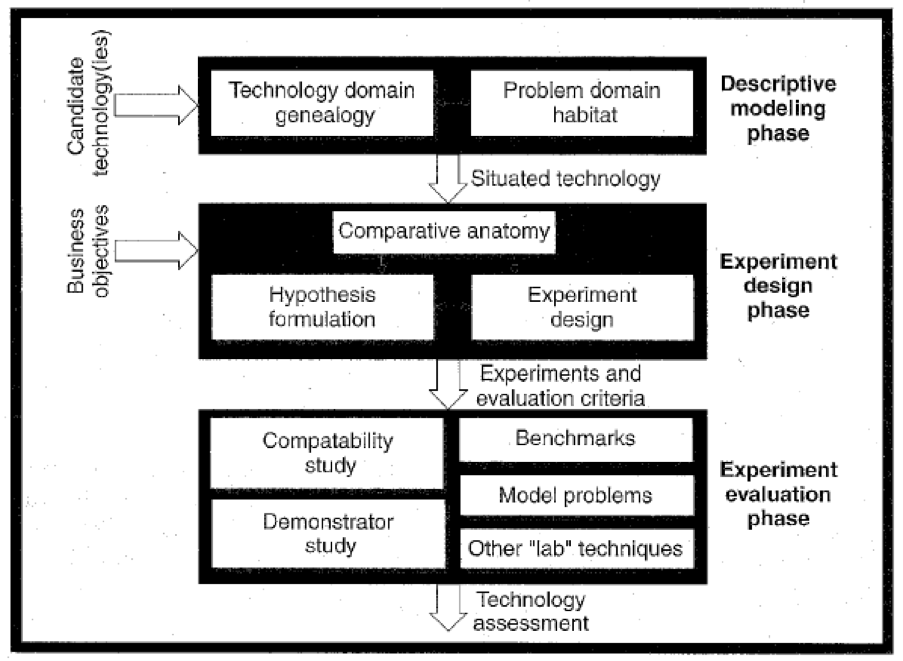
\includegraphics[scale=0.5]{figs/framework.png}
  \caption{Software technology evaluation framework.}
  \label{fig:framework}
\end{figure}


\subsection{Motivation}
we are a motivated lot ,';j

\subsection{Kotlin}

\subsubsection{What is Kotlin?}
Kotlin is a new and open source programming language. It is statically typed programming language that combines object oriented programming with functional programming. That means that one can use both styles of programming interchangeably. Kotlin comes from from JetBrains, the folk behind world's best IDE's. That means it comes from the industry and not academia so it focuses on solving some of the day-to-day tasks developers have to deal with. Kotlin is concise - which means one can expect to reduce amount of code lines written. Safe - it avoids errors like null pointer exceptions. Interoperable - use existing libraries for JVM, Android and the browser. Kotlin compiles down to JVM and Javascript which means that the language can be used for many purposes. Kotlin is also tool-friendly, one can pick any Java IDE or build directly from command line.
\subsubsection{History}
\subsubsection{Functionality} 
\paragraph{•}
\textbf{Expressiveness} - Kotlin's support for type safe builders and delegated properties help to build easy to user abstractions. \paragraph{•}
\textbf{Scalability} - Because of Kotlin's coroutines server side applications can be scaled with minimal hardware requirements. Coroutines suspend computations in a thread without blocking it. Thread blockage is often expensive, with coroutines a library can decide whether to suspend a computation or not. \paragraph{•}
\textbf{Interoperability} - Kotlin is compatible with all frameworks that work with Java. This is great because it lets developers use familiar technology while having the benefits of a modern language. \paragraph{•}
\textbf{Migration}- One can start using Kotlin and still keep older Java codebases. \paragraph{•}
\textbf{Compatibility} - Kotlin is fully compatible with JDK 6. This ensures that it can run on older android devices for example. \paragraph{}
\textbf{Performance} - Kotlin applications run just as fast as Java due to compiling to the same bytecode. Due to inline functions and code using lambdas it runs faster than code written in Java.  
\subsubsection{Where to use Kotlin}
Kotlin is great for server-side applications because of its many functionalities as mentioned in 1.2.3. \paragraph{•}
Kotlin can be used for Android development, it introduces new features while avoiding new restrictions that usually come when introducing a new technology. \paragraph{•}
JavaScript can be targeted by Kotlin and one can also use third party libraries such as JQuery and ReactJS. \paragraph{•}
Kotlin/Native is in undergoing development where compiling Kotlin to Native libraries will not require a VM. \paragraph{•}


\subsection{Kotlin Syntax}
 -On the Syntax of Kotlin (some examples)
 





\section{Android application (Blackjack)}
\label{sec:prototype}

About 5 pages that gives:

\begin{enumerate}
  
\item High-level view of the demonstrator and its purpose.

\item Details of how the demonstrator has been implemented.

\item May involve presentation of code snippets.

\end{enumerate}

The example below shows how you may include code. There are similar
styles for many other langages - in case you do not use Java in your
project. You can wrap the listing into a figure in case you need to
refer to it. How to create a figure was shown in Section~\ref{sec:background}.
  
\lstinputlisting[language=java]{code/BoksVolum.java}

\subsection{Functionality}
functionality of our prototype
 
\subsection{Tools and frameworks}
frameworks we've used
\subsection{Implementation}
\subsubsection{Possibly many subpoints of our different modules}


\section{Experiment results and comaprison to java}
\label{sec:experiments}

About 3 pages that:

\begin{description}

\item[Describes] the software used to establish the test-bed and for implementing the demonstrator prototype.

\item[Explains] what experiments have been done and the results.

\end{description}

For some reports you may have to include a table with experimental
results are other kinds of tables that for instance compares
technologies. Table~\ref{tab:results} gives an example of how to create a table.

\begin{table}
\centering
\begin{tabular}{llrrrrrr}
  Config & Property & States & Edges & Peak & E-Time & C-Time & T-Time
  \\ \hline \hline
22-2 & A   &    7,944  &   22,419  &  6.6  \%  &  7 ms & 42.9\% &  485.7\% \\   
22-2 & A   &    7,944  &   22,419  &  6.6  \%  &  7 ms & 42.9\% &  471.4\% \\   
30-2 & B   &   14,672  &   41,611  &  4.9  \%  & 14 ms & 42.9\% &  464.3\% \\   
30-2 & C   &   14,672  &   41,611  &  4.9  \%  & 15 ms & 40.0\% &  420.0\% \\ \hline
10-3 & D   &   24,052  &   98,671  & 19.8  \%  & 35 ms & 31.4\% &  285.7\% \\   
10-3 & E   &   24,052  &   98,671  & 19.8  \%  & 35 ms & 34.3\% &  308.6\% \\
\hline \hline
\end{tabular}
\caption{Selected experimental results on the communication protocol example.}
\label{tab:results}
\end{table}

\subsection{The switch from Java to Kotlin}
As developers with a background mainly based on java-development, we had to alter most of the habits associated with developing generic java code. T	he most notable change when developing Kotlin copared to java was probably type declarations. whenever you were going to declare a variable, you could quickly find yourself trying to figure out what type it would be, so that you can declare the type of the variable. This is not necessary, as Kotlin only uses var/val when declaring a variable, where the type will be implicit from the type of what the variable is set to. TODO mention lateinit, and type declaration of lateinit variables.
\\
Another interesting pattern to look at is the appearances of semicolons. Coming from java, you are used to enter a semicolon whenever you have finished a statement. Since the semicolons are optional in Kotlin we've decided to avoid using them. Still, looking back at our code, you can find the occasional semicolon on lines where our java-habits likely kicked in.\\
Something that ma have had us hold on to java-practices may be the fact that the language is fully compatible with java, and you can use java-Classes wherever you want to. A result of this is you often end up writing lines exactly as you would in java. As an example, when you want to sort a list in java you may use:
\begin{lstlisting} 
Collections.sort(myList);
\end{lstlisting}
This line would be correct in Kotlin as you can import java.util.Collections and use it with your code. You can use your favorite java package wherever you feel like when using Kotlin, which can lead you to miss out on some of the neat functionalities in kotlin.\\
Fortunately the Android Studio IDE is very helpful when it comes to hints on how to improve your code. Whenever we started writing a nested if-statement, the IDE would offer to convert it to Kotlins {\it When()} syntax. We can take a look at the initial code we wrote for deciding who the winner of a game is, compared to what the IDE altered it to.\\
The initial Code:
\begin{lstlisting}
fun getWinner(player : List<Card>, dealer : List<Card>): EndGameState{
        val playerScore = getScore(player)
        val dealerScore = getScore(dealer)

        if(playerScore > 21){
            return EndGameState.DEALER
        }
        else if(dealerScore > 21){
            return EndGameState.PLAYER
        }
        else{
            if(playerScore > dealerScore) {
                return EndGameState.PLAYER
            }
            else if(playerScore < dealerScore){
                return EndGameState.DEALER
            }
            else{
                return EndGameState.PUSH
            }
        }
} 
\end{lstlisting}
Interesting to note is that this looks a lot like the code in our java-version of the project. However, the IDE advised us to change our Kotlin code to the following format:
\begin{lstlisting}
    fun getWinner(player : List<Card>, dealer : List<Card>): EndGameState{
        val playerScore = getScore(player)
        val dealerScore = getScore(dealer)
        
        return when {
            playerScore > 21 -> EndGameState.DEALER
            dealerScore > 21 -> EndGameState.PLAYER
            else -> when {
                playerScore > dealerScore -> EndGameState.PLAYER
                playerScore < dealerScore -> EndGameState.DEALER
                else -> EndGameState.PUSH
            }
        }
}
\end{lstlisting}
This code looks a lot cleaner, and came as a pleasant surprise from the Android Studio IDE. Active advise from the IDE was definitely helpful when converting from java-development to kotlin-development, as it showed us some neat functionality in kotlin.
\subsection{Ease of development}

\subsection{Boilerplate code}

\subsection{Documentation}

\subsection{Comparison to Java}
\subsubsection{Possibly many subsections here, guys.}


\section{Conclusions}

Concludes on the project, including the technology, its maturity,
learning curve, and quality of the documentation.

The references used throughput the report should constitute a well
chosen set of references, suitable for someone interesting in learning
about the technology.


\bibliographystyle{plain}
\bibliography{report.bib}{}

\end{document}
